%; whizzy paragraph -pdf xpdf -latex ./whizzypdfptex.sh
%; whizzy-paragraph "^\\\\begin{frame}"
% latex beamer presentation.
% platex, latex-beamer でコンパイルすることを想定。 

%     Tokyo Debian Meeting resources
%     Copyright (C) 2009 Junichi Uekawa
%     Copyright (C) 2009 Nobuhiro Iwamatsu

%     This program is free software; you can redistribute it and/or modify
%     it under the terms of the GNU General Public License as published by
%     the Free Software Foundation; either version 2 of the License, or
%     (at your option) any later version.

%     This program is distributed in the hope that it will be useful,
%     but WITHOUT ANY WARRANTY; without even the implied warreanty of
%     MERCHANTABILITY or FITNESS FOR A PARTICULAR PURPOSE.  See the
%     GNU General Public License for more details.

%     You should have received a copy of the GNU General Public License
%     along with this program; if not, write to the Free Software
%     Foundation, Inc., 51 Franklin St, Fifth Floor, Boston, MA  02110-1301 USA

\documentclass[cjk,dvipdfmx,12pt]{beamer}
\usetheme{Tokyo}
\usepackage{monthlypresentation}

%  preview (shell-command (concat "evince " (replace-regexp-in-string "tex$" "pdf"(buffer-file-name)) "&")) 
%  presentation (shell-command (concat "xpdf -fullscreen " (replace-regexp-in-string "tex$" "pdf"(buffer-file-name)) "&"))
%  presentation (shell-command (concat "evince " (replace-regexp-in-string "tex$" "pdf"(buffer-file-name)) "&"))

%http://www.naney.org/diki/dk/hyperref.html
%日本語EUC系環境の時
\AtBeginDvi{\special{pdf:tounicode EUC-UCS2}}
%シフトJIS系環境の時
%\AtBeginDvi{\special{pdf:tounicode 90ms-RKSJ-UCS2}}

\title{OSC 2011 Tokyo/Spring \\東京エリアDebian勉強会}
\subtitle{第74回 2011年3月度}
\author{岩松 信洋 iwamatsu@debian.org\\IRC nick: iwamatsu}
\date{2011年3月5日}
\logo{
\includegraphics[width=8cm]{image200607/openlogo-light.eps}}

\begin{document}

\frame{\titlepage{}}

\section{}
\begin{frame}
 \frametitle{Agenda}
 \begin{itemize}
  \item Debian勉強会とは?
  \item Debian 6.0/squeeze リリース!
  \item 次期リリース Debian 7.0?への動き 
  \item 質疑応答
  \item その他お知らせ
 \end{itemize}
\end{frame}

\begin{frame}{自己紹介}
\begin{itemize}
\item 岩松信洋 (Nobuhiro Iwamatsu)
\item Debian Project Official Developer
\item Debian Bluetooth, Debian Science, Debian Embedded, Debian SuperH
      porter
\item Linux kernel 開発、U-Boot 開発、etc...
\end{itemize}
\end{frame}

\emtext{Debian 勉強会とは?}

\begin{frame}{Debian 勉強会とは?}
\begin{itemize}
\item Debian ユーザとDebian開発者がフェイス・トゥ・フェイスで話し合う場
\item Debian 開発者および開発者予備軍を育成する場
\item Debianの最新情報、バッドノウハウを提供する場
\item 東京(関東)と関西で月に一回開催\\
\url{http://tokyodebian.alioth.debian.org/}
\item お気軽にご参加ください。
\end{itemize}
\end{frame}

\emtext{Debian 6.0 \\ squeeze \\リリース!}

\begin{frame}
 \frametitle{Debian 6.0/squeeze リリース}
\begin{center}
2011年02月06日 Debian 6.0/squeeze リリース!\\

\includegraphics[width=1.0\vsize]{image201103/squeeze.jpg}
\end{center}
\end{frame}


\begin{frame}{今までのリリースサイクル}
\begin{center}
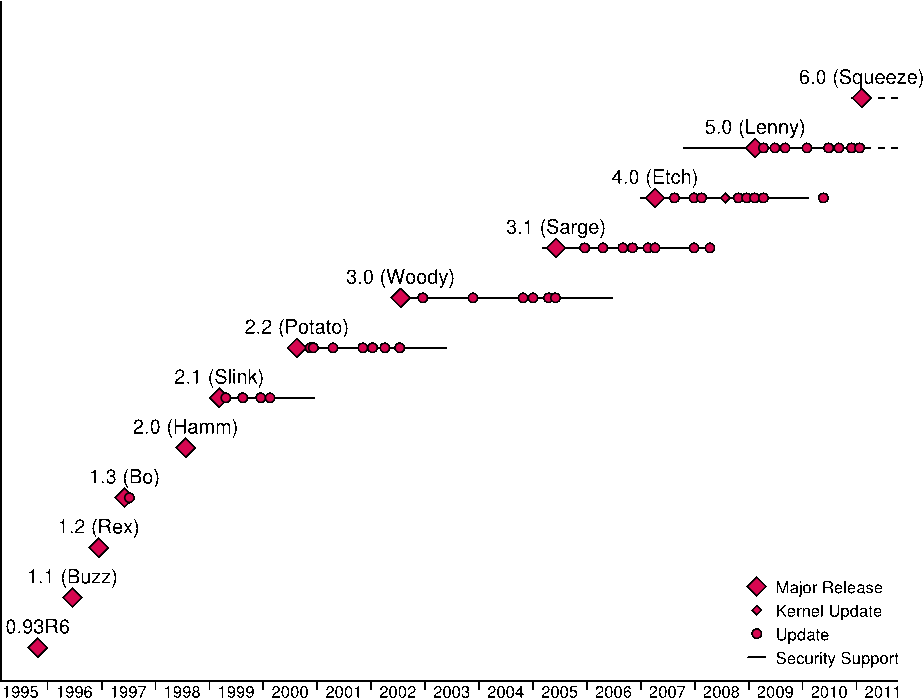
\includegraphics[width=1.1\vsize]{image201103/releases.png}
% \footnote{http://debian.semistable.com/releases.gif}
\end{center}
\end{frame}

\begin{frame}{Debian 6.0 リリースまでの流れ}
\begin{itemize}[<+->] 
\item 2008年09月01日 コードネームアナウンス
\item 2009年02月14日 Debian 5.0/lenny リリース
\item 2009年07月24日 Debconf9 開催 (スペイン・カセレス)
\item 2009年07月29日 タイムベースリリースフリーズの採用を宣言
\item 2009年10月18日 2010年3月にフリーズする予定というアナウンス
\item 2010年02月08日 3月には無理です!というアナウンス
\item 2010年08月01日 Debconf10 開催 (アメリカ・NY)
\item 2010年08月06日 フリーズ宣言
\item 2011年01月13日 Debian Installer 6.0 RC1 リリース
\item 2011年01月22日 Debian Installer 6.0 RC2 リリース
\item 2011年02月06日 Debian 6.0.0 リリース
\end{itemize}

\begin{center}
\Huge %\color{red}2年経ってない!
\end{center}

\end{frame}


\begin{frame}{Debian 6.0 リリースまでの流れ}
\begin{itemize}
\item 2008年09月01日 コードネームアナウンス
\item {\color{red}2009年02月14日 Debian 5.0/lenny リリース}
\item 2009年07月24日 Debconf9 開催 (スペイン・カセレス)
\item 2009年07月29日 タイムベースリリースフリーズの採用を宣言
\item 2009年10月18日 2010年3月にフリーズする予定というアナウンス
\item 2010年02月08日 3月には無理です!というアナウンス
\item 2010年08月01日 Debconf10 開催 (アメリカ・NY)
\item 2010年08月06日 フリーズ宣言
\item 2011年01月13日 Debian Installer 6.0 RC1 リリース
\item 2011年01月22日 Debian Installer 6.0 RC2 リリース
\item {\color{red}2011年02月06日 Debian 6.0.0 リリース}
\end{itemize}
%\pause

\begin{center}
\Huge  \color{red}2年経ってない!
\end{center}

\end{frame}


\begin{frame}{開発者とパッケージ数の推移}
\includegraphics[width=1.2\vsize]{image201103/debian-squeeze-graph00.eps}
\end{frame}

\begin{frame}{Debian 6.0での大きな変更点}
 \frametitle{Debian 6.0での大きな変更点}
\end{frame}

\begin{frame}{Debian 6.0での大きな変更点}
\begin{center}
\large kfreebsd(-i386/-amd64)の追加 (テクノロジープレビュー)


\includegraphics[width=0.7\vsize]{image201103/debian-kfreebsd.png}
\end{center}
\end{frame}


\begin{frame}{Debian 6.0での大きな変更点}
\large Linuxカーネルからnon-free要素を除去
\begin{center}
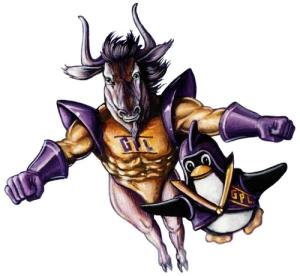
\includegraphics[width=0.7\vsize]{image201103/gnu-linux.jpg}
\end{center}
\end{frame}
% KMSをバックポート
% この成果はもちろん、Linuxカーネルにマージ!


\begin{frame}{Debian 6.0での大きな変更点}
\begin{center}
\large glibc から eglibc に置き換わった
\end{center}
\begin{minipage}[t]{0.45\hsize}

\includegraphics[width=0.4\vsize]{image201103/gnu.png} 
\end{minipage}
\Huge $\rightarrow$
\begin{minipage}[t]{0.40\hsize}

\includegraphics[width=0.40\vsize]{image201103/eglibc-logo.png} 
\end{minipage}
\end{frame}


\begin{frame}{Debian 6.0での大きな変更点}

\large - /bin/sh を bash から dash へ切り替え\\
\large - 新insservとsysv init による依存関係ベースのブートシーケンスへ移
 行

\begin{itemize}
\item 基本システムの bash 依存がなくなった
\item メモリ使用量が小さいため、シェルスクリプトの実行が高速
\item 起動時間が 19秒(bash) から 15秒(dash)に (baseシステムの状態で)\\
(CPU 1GHz(i386) , Memory 512MB の環境)
\item 起動時間が 22秒(bash) から 18秒(dash)に (gnomeをインストールした状態で)
\end{itemize}
\end{frame}

\begin{frame}{Debian 6.0での大きな変更点}
\begin{itemize}%[<+->]
\item GTK1.2、Glib1.2 Gnome1.x 等の古いライブラリを除去
\item arm から、armel への移行。alpha, hppa アーキテクチャをサポート対象
      へ
\item Custom Debian Distributions は Debian Pure Blends に
\end{itemize}

\end{frame}


\begin{frame}{達成されなかった目標}
\begin{center}
しかし達成されなかった目標もある。
\end{center}
\end{frame}


\begin{frame}{達成されなかった目標}%[<+->]
% http://release.debian.org/squeeze/goals.txt

\begin{itemize}
\item multiarchの対応
%多数のアーキテクチャサポートによる、64 ビットマシンへの 32 ビット パッケー
%ジのインストール事情の改善
%kFreeBSD サポート、Debian 初の non-linux アーキテクチャの導入
%dash を新しいデフォルトシェルとしてブート性能を改善し、 依存ベースのブー
%トシステムによるブートプロセスのクリーンアップと 並行処理による性能向上
%を図る
%\item 品質保証 (QA) プロセスをさらに拡張してパッケージの品質向上につなげる。その内容:\\
% \begin{itemize}
% \item 全パッケージについてクリーンインストール、アップグレード及び削除
% \item 基礎的な品質チェックに通らなかったパッケージの自動拒否
% \item ダブルコンパイルのサポート
%\end{itemize}

\item ソースフォーマット 3.0 への移行 
%新しいパッケージ形式(3.0)を策定して、 将来の開発の能率化と圧縮アル
%ゴリズムの改善を図る

% 旧式のライブラリを削除してセキュリティを改善
\item ipv6 の完全サポート
\item ラージファイル(LFS)の完全サポート
%\url{http://bugs.debian.org/cgi-bin/pkgreport.cgi?which=tag\&data=lfs\&archive=no}
\item .la ファイル(libtool アーカイブ)の削除
%\item アーカイブ全体の debug パッケージの自動生成
%Google Summer of Code プロジェクトのインフラへの統合を保留しています。
\item tdeb のサポート
%パッケージの長い説明を翻訳済みパッケージリストに分離して翻訳を促進し、
%また、組み込みシステム向けに小さくしたフットプリントを提供します。 小さ
%くなった Packages ファイルに感謝します(tdeb)。
\item debtags の統合  
%パッケージに複数の属性をタグ付けするシステム、debtags の統合の改善によっ
%てパッケージ選択をもっと簡単に
\item メンテナによってアップロードされたバイナリパッケージの破棄および
      buildd での再ビルド
%\item メンテナによりアップロードされたバイナリパッケージを破棄、再ビルドし、
%制御下の環境でビルドされたパッケージだけを残す。
\end{itemize}
\end{frame}


\begin{frame}{主要パッケージのバージョン}
\begin{itemize}
\item kernel : linux 2.6.32, freebsd 8.1
\item libc : eglibc 2.11
\item GNU Compiler Collection 4.4.5
\item OpenJDK 6b18
\item X server : Xorg X11R7.5
\item Gnome 2.30, KDE 4.4.5, Xfce 4.6 LXDE 0.5.0
\item OpenOffice.org 3.2.1, GIMP 2.6.11
\item Iceweasel 3.5.16 (Mozilla Firefox の商標非使用版)
\item PostgreSQL 8.4.6, MySQL 5.1.49
\item Xen Hypervisor 4.0.1 (dumU 同様に dom0 もサポート)
\item Apache 2.2.16, Samba 3.5.6
\item Python 2.6.6, 2.5.5 and 3.1.3
\item Perl 5.10.1, Ruby 1.8.7.302, 1.9.2.0
\end{itemize}
\end{frame}

\begin{frame}{その他アップデートなど}
\begin{itemize}
\item Debian 17歳 (2010年8月16日)
\item Debian GNU/Linux 4.0 へのセキュリティサポートが終了
\item Debian ベースのディストリビューション間での共同作業インフラを構築
\item backports サービスが公式に
\item パッケージ作業以外での貢献者の受け入れ
\item アーカイブスナップショットサービスが開始
\item Debian volatile が oldstable/stable-updates へ
\end{itemize}

\end{frame}


\emtext{次のリリースは?}

\begin{frame}
 \frametitle{次のリリースはコードネーム:wheezy}
\begin{center}

\includegraphics[width=0.8\vsize]{image201103/toystory_wheezy.jpg}
\end{center}
\pause

\begin{center}
\Large  \color{red}なんてやる気のなさそうな\\ペンギンなんだ!
\end{center}
\end{frame}

\begin{frame}{次のリリースは?}

既に次のリリースに向けて開発が開始!
\begin{itemize}[<+->]
 \item gcc-4.1 を削除。gcc-4.5, 4.6+ へ\\
Go lang が来る!\\
-as-needed, --no-add-needed 対応。\\
 \item eglibc 2.13+ へ
 \item Linux カーネルをアップデート。次の LTS (linux-2.6.37 or 38)サポー
       トへ
 \item jpeg, png, ffmpeg など、主要ライブラリの最新版への移行
 \item Qt3 を削除。Qt4へ完全移行
 \item X.Org 7.6 + にアップデート。wayland は未定。開発は既に開始。
 \item Xfce 4.8 + にアップデート 
 \item OpenOffice.org から LibreOffice へ
 \item debian-ports アーキテクチャのリリースへ。\\
       armhf, powerpcspe, sh4, (m68k?)
 \item その他もろもろ
 \end{itemize}
\end{frame}

\begin{frame}{リリースに向けてのご協力を!}
\begin{itemize}
 \item Debian を使ってください。
 \item squeezeにアップデートしましょう。
 \item バグ報告してください。些細なことでもなんでもOK。\\
2ch とか ブログに書くのは勘弁してください.....。\\
(トラッキングが難しいです)
 \item ドキュメント作成、翻訳に参加してください。\\
翻訳からTypoの指摘歓迎!
 \item パッケージメンテナンス等に興味がある方はサポートします。\\
そのへんにいる Debian 関係者に声をかけてください。
\end{itemize}
\end{frame}


\begin{frame}{質疑応答}
\begin{center}
\Large なにか質問はありますか?
\end{center}
\end{frame}


\begin{frame}{今後のイベント}

\begin{itemize}
 \item 3月 OSC2011 Tokyo Spring CACert keysigning (この後!)
 \item 4月 OSC2011 Kobe (関西エリアDebian勉強会)
 \item 4月 東京エリア Debian勉強会 4月16日(予定)
\end{itemize}
\end{frame}


\begin{frame}{参考文献など}
\begin{itemize}
\item リリースの図 \url{http://debian.semistable.com/releases.gif}
\item リリース目標 \url{http://www.debian.org/News/2009/20090730}
\item リリースノート
      \url{http://www.debian.org/releases/stable/releasenotes}
\item eglibc の絵 \url{http://www.eglibc.org}
\item GNUの絵 \url{http://www.gnu.org}
\item その他 debian-devel@l.d.o
\end{itemize}

\end{frame}


\end{document}

;;; Local Variables: ***
;;; outline-regexp: "\\([ 	]*\\\\\\(documentstyle\\|documentclass\\|emtext\\|section\\|begin{frame}\\)\\*?[ 	]*[[{]\\|[]+\\)" ***
;;; End: ***
